% \Huge

\section{Cosmological Context}

Cosmology has seen many important advances in the last few decades. Piece by piece we are uncovering the history of the universe and it's components. We now know that our galaxy is just one in trillions (\cite{2016ApJ...830...83C}), and part of a rapidly expanding universe.

Our two main observational tools today are the Cosmic Microwave Background (CMB) and Galaxy Surveys. From the CMB we learn about the primordial universe, and Galaxy Surveys uncover the nature and structure of the Universe at late times. The latest surveys like Planck (\cite{2016A&A...594A..13P}), SDSS \todo{ref} or DES \todo{ref} lend strong support to the $\Lambda CDM$ paradigm. Within this Cosmological Standard Model we now understand most of the important events that shaped the history of our Universe and dictate its future. 

The two most important components of this model are arguably Dark Matter and Dark Energy. The two account for a total of about $95\%$ of the matter-energy budget of the universe (e.g. \cite{2016A&A...594A..13P}). We have been able to constrain the properties of the two mysterious components quite well. Most observational probes are consistent with a Cosmological Constant model of dark energy \todo{ref}, but they don't yet exclude other models like quintessence \todo{ref}. On the other hand, the Cold Dark Matter model of a non-interacting (or very weakly interacting) particle that only has gravitational impact is leading on the dark matter side \todo{ref}. However, despite this wealth of knowledge, the nature of the two most important components of the Universe still eludes us.

% % The most important gaps in our knowledge of this Cosmological history are either related to the very early universe (long before the CMB was emitted) or to the evolution of the Universe between recombination and the first galaxies being formed.

% We have very little data on the long period between recombination and until the first stars and galaxies were formed. This long dark age leaves a gap in our ability to study the evolution of primordial perturbation into the structure we see today. 

% The Universe evolved from an initial 
% In this project we will investigate information loss over cosmic evolution. Our aim is to understand how much information about the initial Universe is preserved, and investigate practical ways of recovering it. 

\section{Observational Probes}
\subsection{The Cosmic Microwave Background}

The Cosmic Microwave Background is our main observational tool for studying the early universe. It is the first light emitted in the Universe after recombination, and it encodes plenty of useful information. The CMB is the most perfect black body ever observed (\cite{1999dpf..conf.....W}). Its existence is already a strong proof in support of the Big Bang model. On the other hand, the anisotropies found in the CMB strongly support both the $\Lambda CDM$ paradigm and Inflation.

CMB surveys have measured these anisotropies very accurately (Figure~\ref{fig:1.1}). They are key in understanding the matter distribution in the universe. Before recombination Baryons and Radiation were coupled, so the matter distribution at recombination was imprinted in the CMB distribution. The matter distribution then continued to evolve on its own into the large scale structure we see today. Among the key anisotropies detected in the CMB are Baryon Acoustic Oscillations. This feature is a result of oscillations in the primordial Baryon-Photon plasma. Radiation opposed the collapse of baryonic matter into the potential wells created by collapsing dark matter (which does not interact and is free to collapse). This produced acoustic waves that were imprinted in both the matter distribution (we detect it today in the galaxy distribution) and the radiation distribution (we detect it in the CMB). This probe lends strong support both to the existence of dark matter which plays a key role in their creation, and to that of dark energy (as a cosmological constant) which dictates their evolution at late times.

\begin{figure}
    \centering
    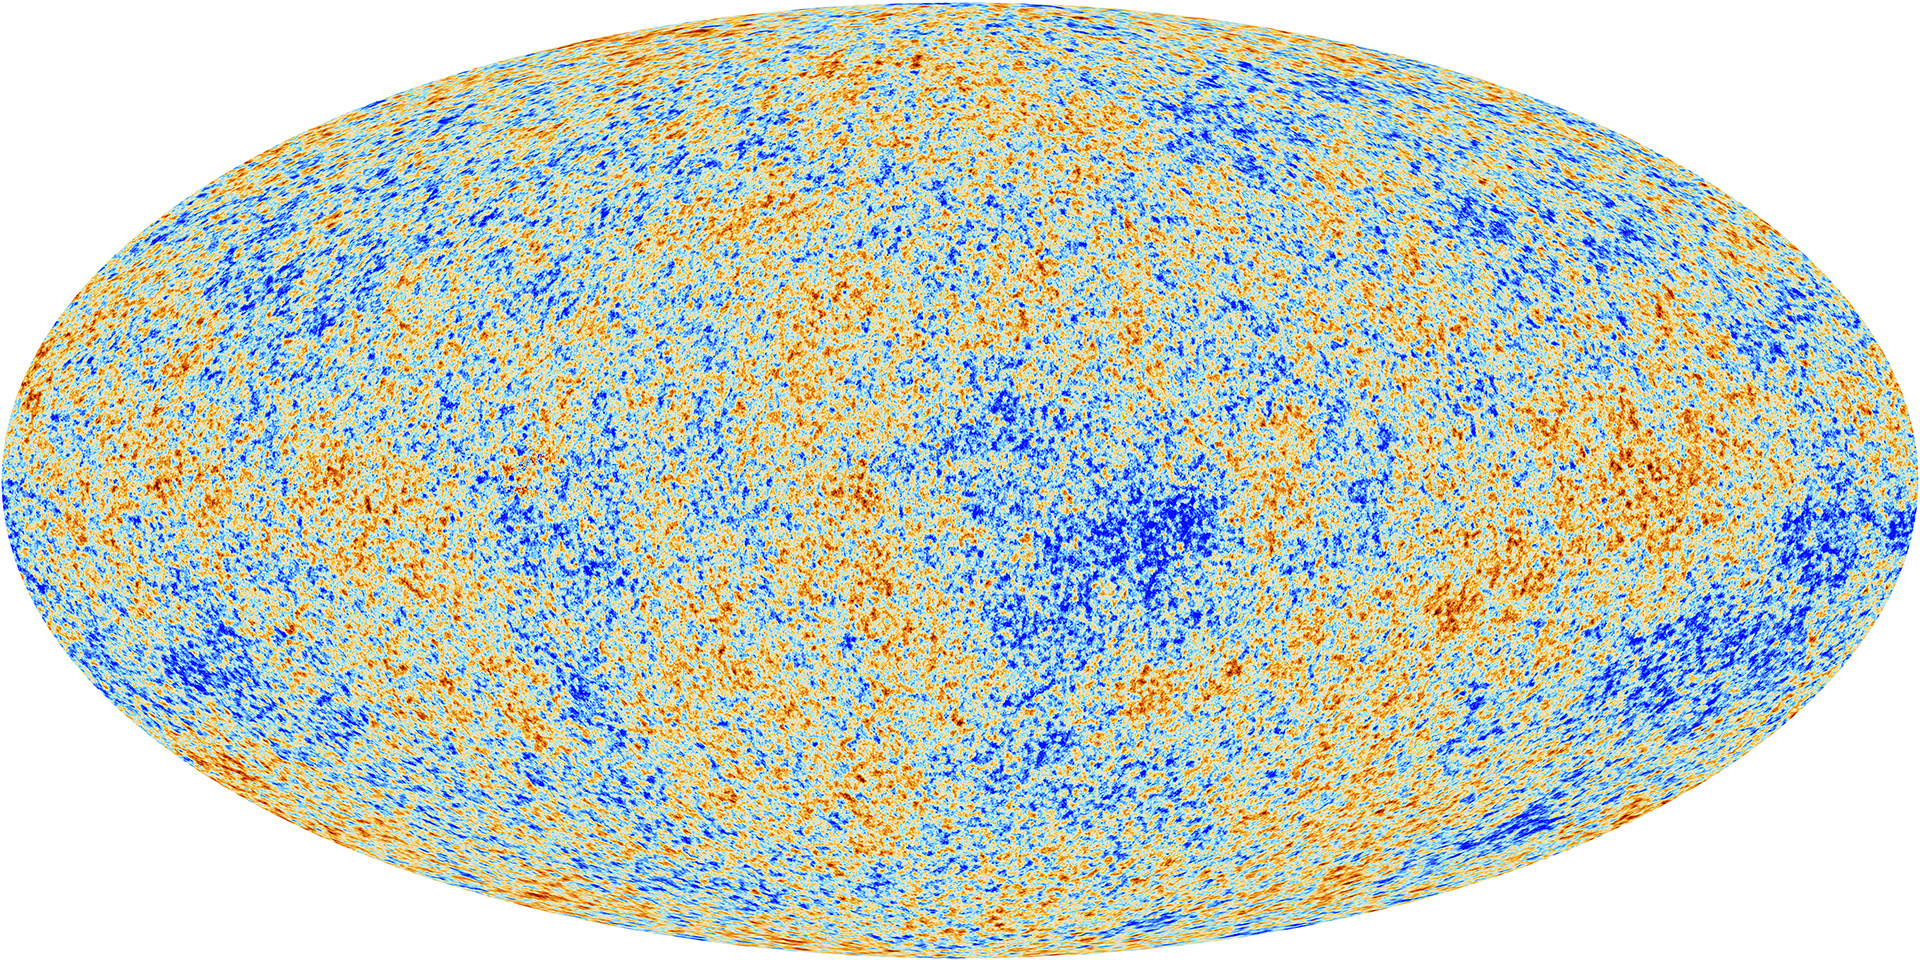
\includegraphics[width=0.9\columnwidth]{images/misc/Planck_CMB.jpg}%
    

    \caption{
    Map of the Cosmic Microwave Background acquired by the Planck Space Telescope (\cite{2016A&A...594A..13P}). After subtracting the effect of our own motion relative to the CMB, the anisotropies only start appearing at $10^{-5} K$. This gives us a glimpse into the primordial matter distribution.
    }
    
    \label{fig:1.1}
\end{figure}

The CMB also has plenty of data in support of Inflation. It shows a uniform, very flat universe that contains mostly gaussian anisotropies. All of these are outcomes of inflation and are hard to explain without it. Of particular interest for us are the gaussian anisotropies. There are many models of inflation \todo{refs!!}, and at the moment we do not have enough precision to distinguish between them. Most models predict some primordial non-gaussianity, however constraining this is key to differentiating between them \todo{ref}.

After the CMB was emitted we enter a period called the Dark Ages. Until the first stars and galaxies formed, the CMB was the only radiation in the Universe. This means we have little to no information about this important era. In it lie the secrets to the formation of the structure we see today in the universe. This shows the main problem of the CMB, it is primarily a 2 dimensional probe showing us the surface of last scattering. While CMB photons do interact with matter on their way to us producing secondary anisotropies, it is far from a complete picture of the evolution of structure.

\subsection{Large Scale Structure and Galaxy Surveys}

Beginning with the first galaxy surveys in the 1980s (\cite{Davis_galaxy_survey}), we started to piece together a picture of the large scale structure of the universe. Galaxies are clustered together and form massive filaments that are separated by huge voids. This web like structure is the result of gravitational collapse of initial perturbations. On the other hand, when looking on the largest scales, the Universe is very uniform.

Recent galaxy surveys like 2dF, SDSS and DES \todo{ref} have brought us a wealth knowledge about the Universe today. They are great tool for studying the universe because, unlike the CMB, we now have a 3 dimensional distribution. Future surveys such as LSST (\cite{2009arXiv0912.0201L}) and DESI (\cite{2013arXiv1308.0847L}) are set to map larger and larger areas of the Universe with ever increasing sensitivity. One of their main objectives is to measure the imprint left by Baryon Acoustic Oscillations in the matter distribution. 

This feature is even more important at these late times, because it was locked on a certain scale after recombination. This means we can use it as a characteristic length scale that evolves with Universe. However, there are some problems that also appear. Firstly, galaxies are biased tracers of the underlying matter distribution (e.g.~\cite{2016arXiv161109787D}). Secondly, non-linear gravitational collapse smears out this feature, reducing the precision of the length scale. As this is a large scale feature, it is however possible to reconstruct it.~\cite{Eisenstein_BAOpeak_reconstruction} argued that most of the contributions to broadening are from super cluster formation and bulk flows. Therefore, Perturbation Theory can be used to perform this reconstruction. Many methods have been proposed to recover this feature. For example,~\cite{1992MNRAS.254..315W} proposed a simple "Gaussianization", while~\cite{1992ApJ...391..443N} and~\cite{1993ApJ...405..449G} introduced a technique based on the success of the Zel'dovich Approximation. More complex methods have also been proposed by~\cite{1999MNRAS.308..763M},~\cite{1997MNRAS.285..793C} and~\cite{2003MNRAS.346..501B}.

These methods have been instrumental in using survey data to its fullest.~\cite{2013PhR...530...87W} estimate that this increase in precision is equivalent to a factor $2-4$ increase in survey size.


% \begin{figure}
%     \centering
%     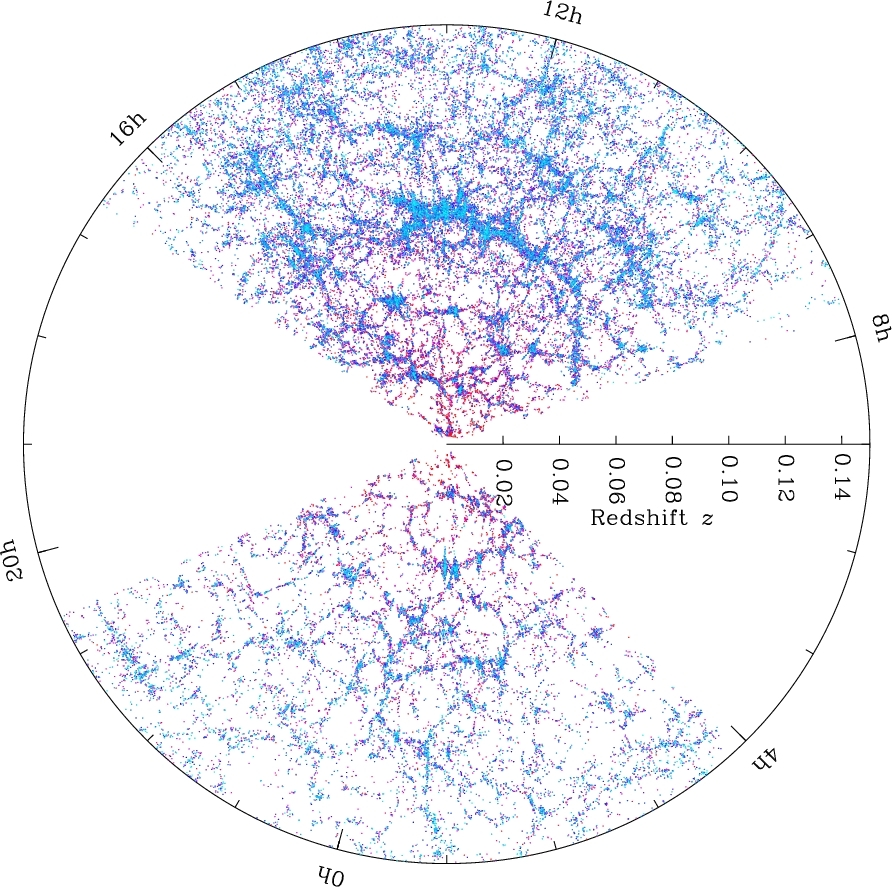
\includegraphics[width=0.9\columnwidth]{images/misc/orangepie.jpg}%
    
%     \caption{
%     Galaxy map from the Sloan Digital Sky Survey.
%     }
    
%     \label{fig:1.2}
% \end{figure}

\section{The Growth of Structure}

In this section we will take a closer look at some of the tools we use to study the growth of structure in the universe. The evolution of primordial perturbations into the structure we detect today is studied analytically using Perturbation Theory (PT). This field can be divided, according to the frame used to study the Universe, into Eulerian PT and Lagrangian PT (LPT). In the Eulerian frame the evolution of the spatial distribution of particles is studied (\cite{Bernardeau_PT}). On the other hand, in the Lagrangian frame, particles are tracked and their evolution with time is studied.

The Eulerian frame has been so widely used to study the growth of perturbations, that we refer to it as Standard Perturbation Theory (e.g. \cite{1983MNRAS.203..345V}, \cite{peebles1980large}). The most popular approach is to consider an irrotational fluid characterized by its overdensity and peculiar velocity distributions (\cite{Carlson_perturbation_theory}). However, this method suffers from divergences at large wavenumbers (on small scales). This lead to a number of extensions meant to bring it under control (\cite{2006PhRvD..73f3519C},~\cite{2008PhRvD..77b3533C}). 

Lagrangian Perturbation Theory has been well developed in the 1990s (\cite{1992MNRAS.254..729B},~\cite{1993MNRAS.264..375B},~\cite{1994MNRAS.267..811B}). However, it has received less attention partly because the method breaks down after shell-crossing (\cite{Carlson_perturbation_theory}). This event will be discussed further in Section 2.2. Recently it has been demonstrated that LPT correctly reproduces the SPT power spectrum, but also even it's linear first order approximation correctly predicts the decay of the correlation between the final (non-linear) and the initial fields (\cite{2008PhRvD..77f3530M},~\cite{2008PhRvD..78h3519M}). As this correlation is the main tool used in this project, our main focus will be on the Lagrangian Frame. 

Once we get into the deeply non-linear regime, these analytic methods break down. Instead we rely on large N-body simulations to continue our study of the evolution of structure. Generally, these simulations are used to help constrain Cosmological theories of the primordial universe or to test perturbation theories. A random initial field with properties based on the CMB and our general understanding of the early universe, is evolved through time until the present. The output of the simulation is then compared to observational data. Simulations like Millennium XXL (\cite{Millennium_XXL}) or Illustris (\cite{Illustris_sim}) gave us an unprecedented insight into structure formation and evolution.

On the other hand, simulations are also used as a laboratory for testing reconstruction methods they give us access to both the initial and the final density fields. We can attempt a reconstruction on the final field and then compare it to the initial field and test how well it worked. 

\section{Recovering Lost Information}

